\documentclass[xcolor=dvipsnames]{beamer}
\usepackage{lmodern}
\usepackage[T1]{fontenc}
\usepackage[english]{babel}
\usepackage[utf8]{inputenc}

\usepackage{manfnt}
\usepackage{wasysym}
\usepackage{listings}
\usepackage{graphicx}
\usepackage{url}
\usepackage{ulem}
\usepackage{marvosym}
\usepackage{skull}
\usepackage{proof}
\usepackage{array}
\usepackage{colortbl}
\setbeamertemplate{navigation symbols}{}

\title[Landslide]{{\bf Coping with Exponential Explosion \\ during Systematic Testing}}
%\subtitle[]{ {\em more clever than } ``\texttt{slaughter cho2}'' {\em since 2011.}}
\author[Ben Blum]{Ben Blum \texttt{(bblum@cs.cmu.edu)} \\ {\small Joint work with Garth Gibson}}

\institute[CMU]{Carnegie Mellon University}
\date[]{2014, June 4}

\setbeamertemplate{footline}{\hspace*{.5cm}\scriptsize{\insertauthor\hspace*{50pt} \hfill\insertframenumber\hspace*{.5cm}}} 

\usecolortheme{seahorse}
\usecolortheme{rose}
\useoutertheme{infolines}

\usecolortheme[named=ForestGreen]{structure}

\newcommand\noob{\mathsf{noob}}
\newcommand\gibs{\mathsf{gibs}}
\newcommand\dps{\mathsf{dps}}
\newcommand\squig\rightsquigarrow
\newcommand\Coloneqq{\mathrel{\mathop{::}}=}
\newcommand\dmg{\text{\Laserbeam}}
\newcommand\delter\delta
\newcommand\alpher\alpha
\newcommand\defnor{\text{ }|\text{ }}

\newcommand\pimp{\mathop{\supset}}
\newcommand\pand{\mathop{\wedge}}
\newcommand\por{\mathop{\vee}}
\newcommand\ptrue{\top}
\newcommand\pfalse{\bot}


\begin{document}
\normalem
\begin{frame}
	\titlepage
\end{frame}

%%%%%%%%%%%%%%%%%%%%%%%%%%%%%%%%%%%%%%%%%%%%%%%%%%%%%%%%%%%%%%%%%%%%%%%%%%%%%%%%
%%%%%%%%%%%%%%%%%%%%%%%%%%%%%%%%%%%%%%%%%%%%%%%%%%%%%%%%%%%%%%%%%%%%%%%%%%%%%%%%
%%%%%%%%%%%%%%%%%%%%%%%%%%%%%%%%%%%%%%%%%%%%%%%%%%%%%%%%%%%%%%%%%%%%%%%%%%%%%%%%

\newcommand\linegap{\vspace{0.2in}}
\newcommand\breakslide[1]{\begin{frame}{} \begin{center} {\Large #1} \end{center} \end{frame}}

\section{Introduction}

% Before intro outline slide, say about this talk words

\subsection{Introduction}

\begin{frame}{Outline}
	\textbf{Intro to Systematic Testing}
	\begin{itemize}
		\item Race condition example
		\item Stress testing
		\item Preemption points and systematic testing
		%\item State space reduction/estimation % part of below
		\item Challenge: Exponential explosion
		%\item State space reduction
		%\item State space estimation
		%\item Iterative context bounding
			% say: survey of the state of the art
	\end{itemize}
	{\bf Landslide}
	\begin{itemize}
		\item Design \& scope
		\item Successes and limitations in 15-410
	\end{itemize}
	\linegap
	% Say: "A way of dealing with this challenge" - w/o details
	{\bf Iterative Deepening}
	\begin{itemize}
			% say: "which basically means..."
		\item Automatically configuring test parameters
			% say: "to save user time and accomodate testing time limits"
		\item Evaluation plan
		\item Limitations

		% Say: A new technique I've been working on to overcome one of systematic testing's inherent weaknesses that can hopefully make Landslide accessible to a wider range of 15-410 students.
	\end{itemize}
\end{frame}

\newcommand\related[1]{\textsuperscript{\em [#1]}}

%%%%%%%%%%%%%% notes on sections / slides %%%%%%%%%%%%%%%%%%%%%%
\newcommand\dontcompilethis[1]{}

%%%%%%%%%%%%%%%%%%%%%%%%%%%%%%%%%%%%%%%%%%%%%%%%%%%%%%%%%%%%%%%%%%%%%%%%%%%%%%%%
%%%%%%%%%%%%%%%%%%%%%%%%%%%%%%%%%%%%%%%%%%%%%%%%%%%%%%%%%%%%%%%%%%%%%%%%%%%%%%%%

\section{Systematic Testing}

\breakslide{Background (Why Systematic Testing?)}

\begin{frame}[fragile]{Case Study}
	\begin{center}
	\begin{verbatim}
	    /* thread_fork system call */
	    int thread_fork()
	    {
	        thread_t *child = construct_new_thread();
	        add_to_runqueue(child);
	        return child->tid;
	    }
	\end{verbatim}
	\end{center}
	\pause

	\begin{itemize}
		\item On exit, child's thread control block (TCB) is freed
		\item Forking thread does use-after-free
		\item Might return garbage instead of thread-ID
	\end{itemize}
\end{frame}

\begin{frame}{Case Study - ``Good'' Interleaving}
	\begin{tabular}{|l|l|l}
		\cline{1-2}
		{\bf Thread 1} & {\bf Thread 2} & \\
		\cline{1-2}
		\texttt{spawn\_new\_thread} && \\
		\cline{1-2}
		\texttt{add\_to\_runqueue} && (new thread) \\
		\cline{1-2}
		\texttt{return child->tid} && (yield to child) \\
		\cline{1-2}
		& \texttt{exit} & \\
		\cline{1-2}
		& (TCB gets freed) & \\
		\cline{1-2}
	\end{tabular}
\end{frame}

\begin{frame}{Case Study - Buggy Interleaving}
	\begin{tabular}{|l|l|l}
		\cline{1-2}
		{\bf Thread 1} & {\bf Thread 2} & \\
		\cline{1-2}
		\texttt{spawn\_new\_thread} && \\
		\cline{1-2}
		\texttt{add\_to\_runqueue} && (new thread + preempted) \\
		\cline{1-2}
		& \texttt{exit} & \\
		\cline{1-2}
		& (TCB gets freed) & (yield to parent) \\
		\cline{1-2}
		\texttt{return child->tid} && (bad!) \\
		\cline{1-2}
	\end{tabular}
\end{frame}

% Say: In 15-410 we teach students to think about thread interleavings and race conditions using these 'tabular' execution traces. But to think about the state space in a way compatible with systematic testing, we'll need to move beyond them...

\begin{frame}{Concurrency Testing Techniques}
	How do we test for concurrency bugs?
	\linegap

	Exercise as many interleavings as possible (given some CPU time budget)
	\linegap

	\textbf{Stress testing}
	\begin{itemize}
		\item Testing kernel code, repeatedly run userspace programs
		\item Relies on randomly-occurring timer interrupts % say: to cause context switches
		\item Exposes race conditions unreliably
		\item Might not find bugs in any bounded time
	\end{itemize}
	\pause
	\linegap

	Moving beyond stress testing: Which {\em preemption points} are important?
\end{frame}

\begin{frame}{Preemption Points}
	\textbf{Preemption points} (PPs) are program locations where a context switch might expose different behaviour
	\linegap

	For case study, ``thread becomes runnable'' \& ``thread exits'' are relevant.
	\linegap

	Considering PPs, state space of interleavings can be viewed as a tree.
	% Say "Let's see what our example program's state space looks like if we use X, Y, and Z PPs."
\end{frame}

\definecolor{thread1}{RGB}{87,172,255}
\definecolor{thread2}{RGB}{255,201,102}

\begin{frame}{Case Study - Execution Tree}
	\begin{center}
		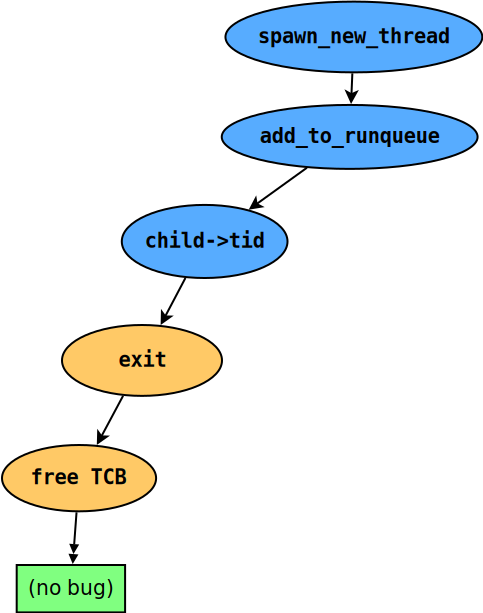
\includegraphics[width=0.7\textwidth]{threadfork0.pdf}
		\hspace{-0.5in} {\tiny 
		\begin{tabular}{c}
			\begin{tabular}{|l|l|}
				\hline
				\cellcolor{thread1} {\bf Thread 1} & \cellcolor{thread2} {\bf Thread 2} \\
				\hline
				{\tt spawn\_new\_thread()} & \\
				\hline
				{\tt add\_to\_runqueue()} & \\
				\hline
				{\tt return child->tid;} & \\
				\hline
				& {\tt exit()} \\
				\hline
				& {\tt <free TCB>} \\
				\hline
			\end{tabular}
			\\ \\ \\ \\ \\ \\ \\ \\
			\\ \\ \\ \\ \\ \\ \\ \\
			\\ \\ \\ \\ \\ \\ \\ \\
			\\ \\ \\ \\ \\ \\ \\ \\
			\\ \\ \\ \\ \\ \\ \\ \\
			\\ \\ \\ \\ \\ \\ \\ \\
			\\ \\ \\ \\ \\ \\ \\ \\
		\end{tabular}
		}
	\end{center}
\end{frame}
\begin{frame}{Case Study - Execution Tree}
	\begin{center}
		\includegraphics[width=0.7\textwidth]{threadfork05.pdf}
		\hspace{-0.5in} {\tiny 
		\begin{tabular}{c}
			\begin{tabular}{|l|l|}
				\hline
				\cellcolor{thread1} {\bf Thread 1} & \cellcolor{thread2} {\bf Thread 2} \\
				\hline
				{\tt spawn\_new\_thread()} & \\
				\hline
				{\tt add\_to\_runqueue()} & \\
				\hline
				{\tt return child->tid;} & \\
				\hline
				& {\tt exit()} \\
				\hline
				& {\tt <free TCB>} \\
				\hline
			\end{tabular}
			\\ \\ \\ \\ \\ \\ \\ \\
			\\ \\ \\ \\ \\ \\ \\ \\
			\\ \\ \\ \\ \\ \\ \\ \\
			\\ \\ \\ \\ \\ \\ \\ \\
			\\ \\ \\ \\ \\ \\ \\ \\
			\\ \\ \\ \\ \\ \\ \\ \\
			\\ \\ \\ \\ \\ \\ \\ \\
		\end{tabular}
		}
	\end{center}
\end{frame}
\begin{frame}{Case Study - Execution Tree}
	\begin{center}
		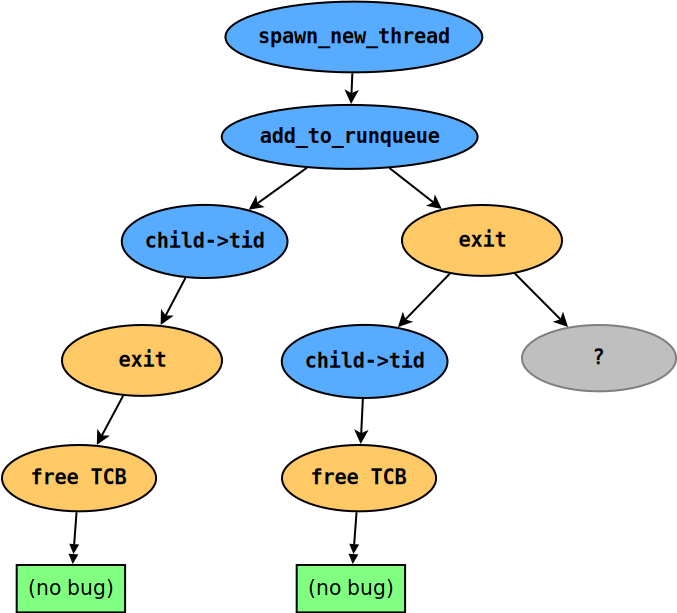
\includegraphics[width=0.7\textwidth]{threadfork1.pdf}
		\hspace{-0.5in} {\tiny 
		\begin{tabular}{c}
			\begin{tabular}{|l|l|}
				\hline
				\cellcolor{thread1} {\bf Thread 1} & \cellcolor{thread2} {\bf Thread 2} \\
				\hline
				{\tt spawn\_new\_thread()} & \\
				\hline
				{\tt add\_to\_runqueue()} & \\
				\hline
				& {\tt exit()} \\
				\hline
				{\tt return child->tid;} & \\
				\hline
				& {\tt <free TCB>} \\
				\hline
			\end{tabular}
			\\ \\ \\ \\ \\ \\ \\ \\
			\\ \\ \\ \\ \\ \\ \\ \\
			\\ \\ \\ \\ \\ \\ \\ \\
			\\ \\ \\ \\ \\ \\ \\ \\
			\\ \\ \\ \\ \\ \\ \\ \\
			\\ \\ \\ \\ \\ \\ \\ \\
			\\ \\ \\ \\ \\ \\ \\ \\
		\end{tabular}
		}
	\end{center}
\end{frame}
\begin{frame}{Case Study - Execution Tree}
	\begin{center}
		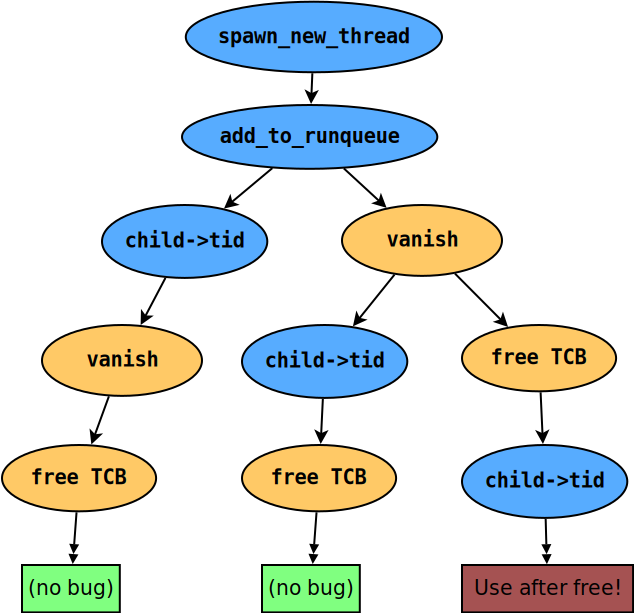
\includegraphics[width=0.7\textwidth]{threadfork.pdf}
		\hspace{-0.5in} {\tiny 
		\begin{tabular}{c}
			\begin{tabular}{|l|l|}
				\hline
				\cellcolor{thread1} {\bf Thread 1} & \cellcolor{thread2} {\bf Thread 2} \\
				\hline
				{\tt spawn\_new\_thread()} & \\
				\hline
				{\tt add\_to\_runqueue()} & \\
				\hline
				& {\tt exit()} \\
				\hline
				& {\tt <free TCB>} \\
				\hline
				{\tt return child->tid;} & \\
				\hline
			\end{tabular}
			\\ \\ \\ \\ \\ \\ \\ \\
			\\ \\ \\ \\ \\ \\ \\ \\
			\\ \\ \\ \\ \\ \\ \\ \\
			\\ \\ \\ \\ \\ \\ \\ \\
			\\ \\ \\ \\ \\ \\ \\ \\
			\\ \\ \\ \\ \\ \\ \\ \\
			\\ \\ \\ \\ \\ \\ \\ \\
		\end{tabular}
		}
	\end{center}
\end{frame}
% Say: "Systematic testing simply means forcing the program to execute each branch of this tree in sequence (and looking for bugs in each one)."


\begin{frame}{Systematic Testing}
	\textbf{Systematic Testing}\related{Godefroid '97}
	\begin{itemize}
		\item Alternative approach to stress testing
		\item Exhaustively exercise {\em all} thread interleavings
		\begin{itemize}
			\item ...around a given set of preemption points
		\end{itemize}
		\item Offers more reliable coverage and better reproducibility
			% say: compared to stress testing
		%\item However, unpredictable relationship between number of PPs and testing time
	\end{itemize}
	\pause
	\linegap

	Which preemption points to use?
	% Say: The tree I showed you was manageable because I knew in advance which preemption points would be relevant to expose the bug.
	\begin{itemize}
		\item Every instruction (exhaustive, but intractable)
		\item Pthread library calls\related{Simsa '10}
		\item Kernel mutex interface calls\related{Blum '12}
		%\item Unprotected shared memory accesses % say: data races
		%\item A new thread becomes runnable
		%\item Voluntary reschedule (e.g. \texttt{yield}, \texttt{cond\_wait})
		%\item Synchronization primitives
	\end{itemize}

\end{frame}

%%%%%%%%%%%%%%%%%%%%%%%%%%%%%%%%%%%%%%%%%%%%%%%%%%%%%%%%%%%%%%%%%%%%%%%%%%%%%%%%
%%%%%%%%%%%%%%%%%%%%%%%%%%%%%%%%%%%%%%%%%%%%%%%%%%%%%%%%%%%%%%%%%%%%%%%%%%%%%%%%

\section{Exponential Explosion}

\breakslide{How does systematic testing scale \\ with more preemption points?}

\breakslide{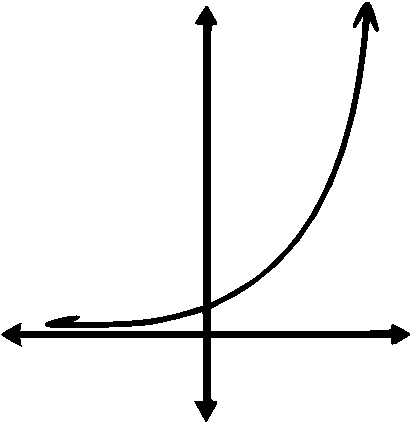
\includegraphics[width=0.40\textwidth]{exponential-curve.pdf}}

\begin{frame}{State Space Reduction}
	Dynamic Partial Order Reduction\related{Flanagan '05}
	\begin{itemize}
		\item Identifies and prunes equivalent interleavings
		\item Analyzes memory accesses between threads to identify independence
		%\item Requires depth-first search of execution tree
	\end{itemize}
	\pause
	\begin{center}
		\includegraphics[width=0.55\textwidth]{dpor.pdf}
	\end{center}
	% Say: DPOR makes some infeasible -> feasible, but some infeasible are still infeasible. To know the difference? transition...

	%Stable Multithreading\related{Cui '13}
	%\begin{itemize}
	%\end{itemize}
\end{frame}

\begin{frame}{State Space Estimation}
	State space estimation\related{Simsa '12} can guess state space size in advance
	\begin{itemize}
		\item Uses known branches as heuristic to guess total tree size
			% say: something more lucid :(
		\item Estimate improves as more state space is explored
		\item Allows user to guess whether completion is feasible
	\end{itemize}
	%\pause
	%\linegap

	%[picture goes here]
	% no picture.
	% picture status: no.
\end{frame}

%\begin{frame}{Iterative Context Bounding\related{Musuvathi 07}}
%	Insight: Most bugs can be exposed with very few preemptions.
%	% say: presenting this specific one because it's most similar to
%	\begin{itemize}
%		\item Explore branches with fewer preemptions first.
%		\item More likely to find bugs sooner, if they exist
%		\item Just as likely to fail to complete too-large state spaces
%	\end{itemize}
%
%	% gr4fix
%\end{frame}

\begin{frame}{Remaining Challenges}
	State-of-the-art systematic testing can {\em mitigate} exponential explosion.
	%\begin{itemize}
	%	\item Reduce testing time exponentially by pruning redundant branches
	%	\item Inform users of total expected testing time
	%		% say: so they can manage testing resources
	%		% by only running tests that are more likely to complete
	%\end{itemize}
	%but still cannot:
	%\begin{itemize}
	%	\item Control total testing time to fit in a given time budget
	%	%\item Automatically decide which preemption points are valuable
	%		% haha-never
	%\end{itemize}
	\linegap

	However...
	\begin{itemize}
		\item With too many preemption points, it still fails
		\item Which PPs are ``good'' differs for each test case.
		\item Relationship between PPs and testing time is unpredictable.
	\end{itemize}
	\pause
	\linegap

	Next: Students who could benefit from systematic testing, if only it were automatic.

	% Say: "In the next section I'll talk about my experience working with students who could potentially benefit from systematic testing, which motivates the need for an automated solution to preemption points.
\end{frame}

%%%%%%%%%%%%%%%%%%%%%%%%%%%%%%%%%%%%%%%%%%%%%%%%%%%%%%%%%%%%%%%%%%%%%%%%%%%%%%%%
%%%%%%%%%%%%%%%%%%%%%%%%%%%%%%%%%%%%%%%%%%%%%%%%%%%%%%%%%%%%%%%%%%%%%%%%%%%%%%%%

\section{Landslide}

\breakslide{Landslide}

\begin{frame}{Overview}
	Landslide: A systematic testing tool for 15-410 Pebbles projects
	\linegap

	15-410: Operating System Design and Implementation
	\begin{itemize}
		\item Pebbles: a small UNIX-like kernel specification
		\item Students implement a userspace thread library and a kernel
		\item Both projects done in 2-person teams
		\item Wind River Simics\textsuperscript{TM}, an x86 simulator, aids development/debugging
	\end{itemize}
	\pause
	\linegap

	Project history
	\begin{itemize}
		%\item Began as 5th-year MS project with Garth Gibson, Jiri Simsa
		\item Tested Pebbles kernels, with user-provided annotations
		\item Recently, fully-automatic instrumentation for thread libraries
	\end{itemize}
\end{frame}

\begin{frame}{Landslide Design}
	As a Simics module, Landslide intercepts:
	\begin{itemize}
		\item Every instruction executed
			% say: useful for modeling the kernel/thrlib's behaviour
		\item Every memory address read/written
			% say: useful for checking memory/heap errors
	\end{itemize}
	\pause
	\linegap

	Navigating the state space
	\begin{itemize}
		\item At each preemption point:
		\begin{itemize}
			\item Injects timer interrupts to control thread scheduling
		\end{itemize}
		\item At end of each iteration (i.e., each interleaving pattern):
		\begin{itemize}
			\item Uses Simics reverse-execution to rewind machine state
		\end{itemize}
	\end{itemize}
\end{frame}

\begin{frame}{Landslide Design}
	\begin{center}
		\includegraphics[width=0.6\textwidth]{landslide.pdf}
	\end{center}
\end{frame}

\newcommand\hilight[2]{\color{#1}#2\color{black}}
\definecolor{olivegreen}{RGB}{0,127,0}
\definecolor{brickred}{RGB}{192,0,0}
\begin{frame}{Landslide Design}
	Identifying bugs
	\begin{itemize}
		\item False-negative-oriented approach % say: "that is, it doesn't flag suspicious behaviours, only behaviours like crashes / segfaults that are obviously wrong"
		\item Assertion failure, use-after-free, deadlock, memory leak, infinite loop
	\end{itemize}
	\pause
	\linegap

	{\small
        \begin{tabular}{l}
        \texttt{\hilight{brickred}{USE AFTER FREE - read from 0x199630 at eip 0x104209}} \\
        %\texttt{Heap contents:~\{...\}} \\
        \texttt{[0x199630 | 4140] was allocated by TID~3 at (...)} \\
        \texttt{~~~~~~~~~~~~~~~~~~~~~~and freed by TID~4 at (...)} \\
        \texttt{\hilight{brickred}{**** A bug was found! Preemption trace follows. ****}} \\
        \texttt{\hilight{olivegreen}{1:~~TID 3 -{}-> TID 4}} \\
	\texttt{~~~~TID 3 at 0x10c25a in \hilight{blue}{timer\_interrupt()},} \\
	\texttt{~~~~~~~~~~~~~0x1041f4 in \hilight{blue}{thread\_fork()}} \\
        %\texttt{~~~~~~~~~~~~0x10362b in \hilight{blue}{thread\_fork\_wrapper}} \\
        \texttt{\hilight{olivegreen}{2:~~TID 4 -{}-> TID 3}} \\
	\texttt{~~~~TID 4 at 0x105a10 in \hilight{blue}{context\_switch()},} \\
	\texttt{~~~~~~~~~~~~~0x104681 in \hilight{blue}{yield()},} \\
	\texttt{~~~~~~~~~~~~~0x104570 in \hilight{blue}{exit()}} \\
        %\texttt{~~~~~~~~~~~~0x103708 in \hilight{blue}{vanish\_wrapper}} \\
        \texttt{\hilight{olivegreen}{Current stack:}}\\
	\texttt{~~~~TID 3 at 0x104209 in \hilight{blue}{thread\_fork()}} \\
        %\texttt{~~~~~~~~~~~~0x10362b in \hilight{blue}{thread\_fork\_wrapper}}
        \end{tabular}
	}
\end{frame}

\begin{frame}{Experience}
	15-410 student feedback
	\begin{itemize}
		\item Recruited students to volunteer near end of kernel project
		\item Provided advice to help annotation, but not to help debug
		\item Majority of groups found previously-unknown races
	\end{itemize}
	\pause
	\linegap

	Limitations
	\begin{itemize}
		\item Students spent \textasciitilde{}2 hours annotating kernels
		\item After annotation, 30-60 min configuring preemption points
			% say: ...before finding & analyzing bugs
		\item Selection bias: only students with free time volunteered
	\end{itemize}
	% Say: reducing annotation effort is just engineering, but the need for
	% the tool to automatically infer & insert "good" preemption points
	% motivates my new technique [of iterative deepening].
\end{frame}

\breakslide{How can systematic testing be as automatic as stress testing, for students in 15-410?}

\begin{frame}{Iterative Deepening in Chess}
	Analogous problem: computer chess
	\begin{itemize}
		\item Depth-first search
		\item Each iteration limited by constant maximum branch depth
		\item CPU time budget fixed in advance
		%\item Unpredictable relationship between depth and time
	\end{itemize}
	\pause
	\linegap
	Repeat iterations of DFS, increasing max depth, until time is exhausted.
\end{frame}

\begin{frame}{Iterative Deepening in Landslide}
	Repeat state space explorations, adding preemption points, until time is exhausted.
	\pause
	\vspace{0.29in}
	\begin{center}
		\includegraphics[width=0.25\textwidth]{tree0.pdf}
	\end{center}
\end{frame}

\begin{frame}{Iterative Deepening in Landslide}
	Repeat state space explorations, adding preemption points, until time is exhausted.
	\vspace{0.15in}
	\begin{center}
		\begin{tabular}{cc}
			\includegraphics[width=0.35\textwidth]{tree1.pdf} &
			\includegraphics[width=0.35\textwidth]{tree2.pdf}
		\end{tabular}
	\end{center}
\end{frame}


\begin{frame}{Iterative Deepening in Landslide}
	Repeat state space explorations, adding preemption points, until time is exhausted.
	\begin{center}
		\includegraphics[width=0.5\textwidth]{tree3.pdf}
	\end{center}
	% say: and depending on your time budget, you might decide that you expect this one to be feasible, or you might fall back to a smaller state space from before.
\end{frame}
\begin{frame}{Iterative Deepening Challenges}
	How best to use state space estimates to predict testing time?
		% say: As we saw when I discussed estimation, accuracy improves as state space coverage increases. So there will be a tradeoff...
	\begin{itemize}
		\item Estimate quality improves as state space coverage increases
		\item Wait longer each iteration before using estimate: More accurate
		\item Wait less each iteration before using estimate: More time saved
	\end{itemize}
	\pause
	\linegap

	Which preemption points matter more? % say i.e., which are most likely to find bugs? conversely, which provide most meaningful guarantee if no bug is found?
	% say: relying on human intuition, how can we reproduce that automatically
	\begin{itemize}
		\item Use same default set as before (mutex/scheduler operations)
		\item Look for unsafe shared memory accesses to identify new candidates
		%\item Assign heuristic priorities to each class of preemption points
	\end{itemize}
\end{frame}

\begin{frame}{Evaluation}
	Can experienced TAs use systematic testing to grade more accurately?
	\begin{itemize}
		\item Compare with Fritz, 15-410 stress-testing framework
		\item Run each on several semesters of projects, compare bugs found
	\end{itemize}
	\pause
	\linegap

	Can students use systematic testing as easily as stress testing?
	\begin{itemize}
		\item Offer fully-automatic Landslide during thread library project
		\item Compare quality of student submissions to past semesters
		\item Survey students for time spent debugging, learning the tool, etc.
	\end{itemize}
\end{frame}

\begin{frame}{Limitations / Future Work}
	Individually-long-running tests for resource exhaustion scenarios
	\begin{itemize}
		\item Systematic testing relies on short test case iterations
		\item Some program behaviours only arise, e.g., when \texttt{malloc()} fails
	\end{itemize}
	\pause
	\linegap

	Reliance on imperfect techniques as building blocks
	\begin{itemize}
		\item State space estimates
			%\begin{itemize}
				%\item Accuracy is often dependent on exploration ordering
			%\end{itemize}
		\item Using shared memory accesses as preemption points
			\begin{itemize}
				\item False positives (benign access pairs) can cause unnecessary work
				\item Especially likely when testing concurrency primitives
			\end{itemize}
	\end{itemize}
	\pause
	\linegap

	Some reliance on human intuition remains
	\begin{itemize}
		\item Test authors may need annotations to influence preemption points
			% say: Anticipate will need annotations for author of test suite
	\end{itemize}
\end{frame}

\section{Conclusion}

\breakslide{Wrap-Up}

\begin{frame}{Conclusion}
	\textbf{Systematic testing}: an alternative to stress testing
	\begin{itemize}
		\item Offers more reliable, exhaustive coverage of thread interleavings
		\item Parameterized by a set of {\bf preemption points}
		\item Testing time is exponential in number of PPs % say: and unpredictable
		\item State-of-the-art can mitigate explosion, but still vulnerable
	\end{itemize}
	\linegap

	{\bf Iterative deepening} of preemption points
	\begin{itemize}
		\item Use state space estimation to inform testing strategy
		\item Allows systematic testing to predictably fit CPU time budgets
		\item In Landslide, may offer a new testing/debugging platform for 15-410
	\end{itemize}
\end{frame}

\breakslide{\begin{center} Questions? \\ \vspace{0.3in} \includegraphics[width=0.6\textwidth]{3word-questions.png} \end{center}}

% TODO: POST-PRACTICE bonus slide for CHESS ICB
% TODO: POST-PRACTICE bonus slide for THIS IS WHAT THE REFRANCE



\end{document}
